\addcontentsline{toc}{chapter}{Занятие 2. Характеристики случайного процесса}
\chapter*{Занятие 2. Характеристики случайного процесса}

\addcontentsline{toc}{section}{Контрольные вопросы и задания}
\section*{Контрольные вопросы и задания}

\subsubsection*{Приведите определение случайного процесса.}

Случайный процесс $ \xi \left( t \right), \, t \in T$ ---
это параметризированная совокупность случайных величин.

\subsubsection*{Что называют конечномерными распределениями случайного процесса?}

$ \left\{ \mu_{t_1, \dotsc, t_n}; \, t_1, \dotsc, t_n \in T, \, n \geq 1 \right\} $ ---
набор конечномерных распределений процесса $ \xi $, где $ \mu_{t_1, \dotsc, t_n}$ ---
распределение вектора $ \left( \xi \left( t_1 \right), \dotsc, \xi \left( t_n \right) \right) $ в
$ \mathbb{R}^n$,
то есть для борелевского
$ \Delta \in \mathcal{B} \left( \mathbb{R}^n \right), \,
  \mu_{t_1, \dotsc, t_n} \left( \Delta \right) =
  P \left\{
    \left( \xi \left( t_1 \right), \dotsc, \xi \left( t_n \right) \right) \in \Delta
  \right\} $.

\subsubsection*{Приведите определение функции математического ожидания,
                дисперсии и ковариационной функции случайного процесса.}

$m \left( t \right) = M \xi \left( t \right), \, t \in T$ --- функция среднего.

$D \xi \left( t \right), \, t \in T$ --- функция дисперсии.

$K \left( t, s \right) =
  M \left[ \xi \left( t \right) - m \left( t \right) \right] \cdot
  \left[ \xi \left( s \right) - m \left( s \right) \right], \, t, s \in T$ ---
функция ковариации.

\addcontentsline{toc}{section}{Аудиторные задачи}
\section*{Аудиторные задачи}

\subsubsection*{2.2}

\textit{Задание.}
Пусть
$$ \xi \left( t \right) =
  X \cdot e^{-t}, \,
  t > 0,$$
где $X$ --- случайная величина,
которая имеет нормальное распределение с параметрами $a, \, \sigma^2$.
Найдите математическое ожидание, дисперсию,
ковариационную функцию и одномерную плотность распределения случайного процесса
$ \xi =
  \left\{ \xi \left( t \right), \, t > 0 \right\} $.

\textit{Решение.}
Сейчас $T = \left( 0, \infty \right) $.

Случайная величина $X$ имеет распределение $N \left( a, \sigma^2 \right) $.
Нужно найти $M \xi \left( t \right) = m \left( t \right), \, D \xi \left( t \right) $,
ковариационную функцию $K \left( t, s \right) $ и одномерную плотность распределения
$p_{ \xi } \left( t \right) $.

Найчнём с математического ожидания
$$m \left( t \right) =
  M \left( X \cdot e^{-t} \right) =
  e^{-t} MX =
  e^{-t} \cdot a.$$

Далее ---
функция дисперсии $D \xi \left( t \right) = D \left( X \cdot e^{-t} \right) = e^{-2t} \cdot DX$.
Дисперсия $X$ --- известная: $e^{-2t} \cdot DX = e^{-2t} \cdot \sigma^2$.

Далее ---
ковариационная функция
$$K \left( t, s \right) =
  M \left[ \xi \left( t \right) - m \left( t \right) \right] \cdot
  \left[ \xi \left( s \right) - m \left( s \right) \right] =
  cov \left[ \xi \left( t \right), \xi \left( s \right) \right].$$
Вместо $ \xi \left( t \right), \, \xi \left( s \right) $ подставляем их значения
$$cov \left[ \xi \left( t \right), \xi \left( s \right) \right] =
  cov \left( Xe^{-t}, Xe^{-s} \right).$$
Множители выносятся
$$cov \left( Xe^{-t}, Xe^{-s} \right) =
  e^{-t - s} cov \left( X, X \right) =
  e^{-t - s} DX =
  e^{-t - s} \sigma^2.$$

Последнее ---
это плотность $ \xi \left( t \right) \sim N \left( e^{-t} a, \, e^{-2t} \sigma^2 \right) $.

Нужно написать нормальную плотность с заданными математическим ожиданием и дисперсией
$$p_{ \xi \left( t \right) } \left( x \right) =
  \frac{1}{ \sqrt{2 \pi e^{-2t} \sigma^2}} \cdot
  e^{- \frac{ \left( x - e^{-t} a \right)^2}{2e^{-2t} \sigma^2}}.$$

Траектория процесса изображена на рисунке \ref{fig:22}
и имеет разный вид в зависимости от значения случайной величины $X$.

\begin{figure}[h!]
  \centering
  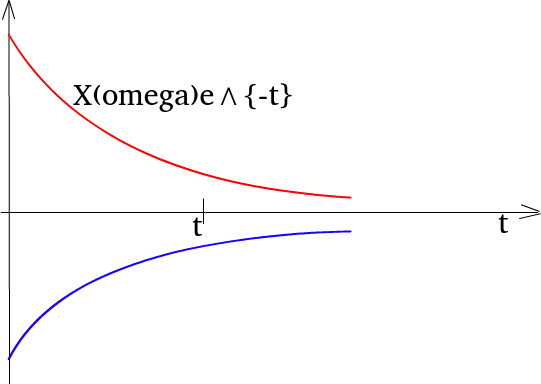
\includegraphics[width=.4\textwidth]{./pictures/2_2.png}
  \caption{Траектория процесса}
  \label{fig:22}
\end{figure}

\subsubsection*{2.3}

\textit{Задание.}
Пусть
$$ \xi \left( t \right) =
  e^{-Xt}, \,
  t > 0,$$
где $X$ --- случайная величина, которая имеет показательное распределение с параметром $ \lambda $.
Запишите конечномерные распределения случайного процесса
$ \left\{ \xi \left( t \right), \, t > 0 \right\} $.
Найдите его математическое ожидание, дисперсию и ковариационную функцию.

\textit{Решение.}
$ \xi \left( t \right) = e^{-Xt}$, где $X \sim Exp \left( \lambda \right), \, t > 0$.

Нужно найти $m \left( t \right), \, K \left( t, s \right) $, конечномерные распределения.

Найдём математическое ожидание в момент $t$.
По определению
$$m \left( t \right) =
  Me^{-Xt} =
  \int \limits_0^{+ \infty } \lambda e^{- \lambda x} e^{-Xt} dX =
  \frac{ \lambda }{ \lambda + t}.$$
Траектории такого процесса изображены на рисунке \ref{fig:23}: чем больше $X$,
тем быстрее эта функция убывает.

\begin{figure}[h!]
  \centering
  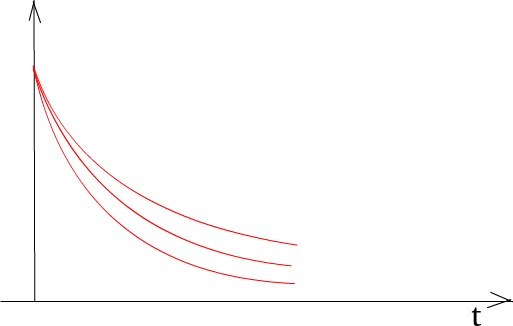
\includegraphics[width=.4\textwidth]{./pictures/2_3.png}
  \caption{Траектория процесса}
  \label{fig:23}
\end{figure}

Ковариационная функция считается по определению
$$K \left( t, s \right) =
  M \xi \left( t \right) \xi \left( s \right) - M \xi \left( t \right) M \xi \left( s \right) =
  Me^{-Xt - Xs} - \frac{ \lambda }{ \lambda + t} \cdot \frac{ \lambda }{ \lambda + s}.$$
Подставим найденное значение фунцкии математического ожидания
$$Me^{-Xt - Xs} - \frac{ \lambda }{ \lambda + t} \cdot \frac{ \lambda }{ \lambda + s} =
  \frac{ \lambda }{ \lambda + t + s} -
  \frac{ \lambda^2}{ \left( \lambda + t \right) \left( \lambda + s \right) }.$$

Считаем функцию распределения случайного вектора
$ \left( \xi \left( t_1 \right), \dotsc, \xi \left( t_n \right) \right) $ --- рис. \ref{fig:231}.

\begin{figure}[h!]
  \centering
  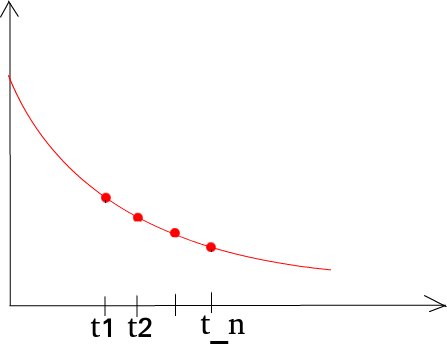
\includegraphics[width=.4\textwidth]{./pictures/2_3_1.png}
  \caption{Выбираем точки, в которых ищем распределение случайного процесса}
  \label{fig:231}
\end{figure}

$F_{ \left( \xi \left( t_1 \right), \dotsc, \xi \left( t_n \right) \right) }
  \left( \vec{x} \right) =
  P \left\{ \xi \left( t_1 \right) \leq x_1, \dotsc, \xi \left( t_n \right) \leq x_n \right\} $.
Вместо $ \xi $ напишем формулу
$P \left\{ \xi \left( t_1 \right) \leq x_1, \dotsc, \xi \left( t_n \right) \leq x_n \right\} =
  P \left( e^{-Xt_1} \leq x_1, \dotsc, e^{-Xt_n} \leq x_n \right) $.
Величины зависимы, потому что все они выражаются через $X$.
Все неравенства решаем относительно $X$
$$P \left( e^{-Xt_1} \leq x_1, \dotsc, e^{-Xt_n} \leq x_n \right) =
  P \left\{ X \geq -\frac{ln \, x_1}{t_1}, \dotsc, X \geq -\frac{ln \, x_n}{t_n} \right\}.$$
Перепишем через максимум
$$P \left\{ X \geq -\frac{ln \, x_1}{t_1}, \dotsc, X \geq -\frac{ln \, x_n}{t_n} \right\} =
  P \left\{
    X \geq \max \left( -\frac{ln \, x_1}{t_1}, \dotsc, -\frac{ln \, x_n}{t_n} \right) \right\}.$$
Обозначим максимум буквой $m$
$$P \left\{
    x \geq \max \left( -\frac{ln \, x_1}{t_1}, \dotsc, -\frac{ln \, x_n}{t_n} \right) \right\} =
  \int \limits_m^{+\infty } \lambda e^{-\lambda X} dX =
  -\left. e^{-\lambda X} \right|_m^{+\infty}.$$
На бесконечности получаем ноль
$$-\left. e^{-\lambda X} \right|_m^{+\infty} =
  e^{-\lambda m} =
  e^{-\lambda \max \left( ln \, x_1^{-\frac{1}{t_1}}, \dotsc, ln \, x_n^{-\frac{1}{t_n}} \right) }.$$
Выносим логарифм
$$e^{-\lambda \max \left( ln \, x_1^{-\frac{1}{t_1}}, \dotsc, ln \, x_n^{-\frac{1}{t_n}} \right) } =
e^{-\lambda ln \max \left( x_1^{-\frac{1}{t_1}}, \dotsc, x_n^{-\frac{1}{t_n}} \right) }.$$
Экспонента и логарифм уничтожают друг друга
$$e^{-\lambda ln \max \left( x_1^{-\frac{1}{t_1}}, \dotsc, x_n^{-\frac{1}{t_n}} \right) } =
  \max \left( x_1^{-\frac{1}{t_1}}, \dotsc, x_n^{-\frac{1}{t_n}} \right)^{-\lambda } =
  \min \left( x_1^{ \frac{ \lambda }{t_1}}, \dotsc, x_n^{ \frac{ \lambda }{t_n}} \right).$$

Все выкладки были законные, только когда $0 < x_1, \dotsc, x_n < 1$.

Плотности у такого векора $ \left( \xi \left( t_1 \right), \dotsc, \xi \left( t_n \right) \right) $
быть не может, потому что
$ \xi \left( t_1 \right)^{ \frac{1}{t_1}} =
  e^{-X} =
  \xi \left( t_2 \right)^{ \frac{1}{t_2}}$.
Сейчас у нас только одна случайная величина.
Это можно переписать как
$ \xi \left( t_2 \right) = \xi \left( t_1 \right)^{ \frac{t_2}{t_1}}, \,
  y = x^{ \frac{t_2}{t_1}}.$

С вероятностью 1 $ \left( \xi \left( t_1 \right), \xi \left( t_2 \right) \right) \in L$ ---
рис. \ref{fig:232}.

\begin{figure}[h!]
  \centering
  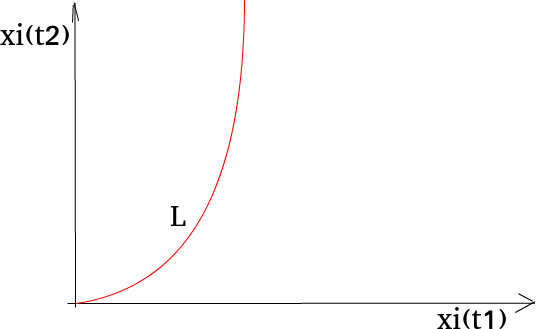
\includegraphics[width=.5\textwidth]{./pictures/2_3_2.png}
  \caption{$y = x^{ \frac{t_2}{t_1}}$}
  \label{fig:232}
\end{figure}

Значения вектора всегда попадают на такую линию.
Площадь кривой --- ноль.

Плотность --- производная от функции распределения, а минимум нельзя дифференцировать.

\subsubsection*{2.4}

\textit{Задание.}
Рассмотрим случайный процесс
$$X \left( t \right) =
  A \cos \left( \varphi + \lambda t \right),$$
где $A$ и $ \varphi $ являются независимыми случайными величинами такими, что $MA^2 < \infty $,
а $ \varphi $ имеет равномерное распределение на отрезке $ \left[ 0, 2 \pi \right] $.
Найдите математическое ожидание и ковариационную функцию процесса
$$ \left\{ X \left( t \right), \, t \geq 0 \right\}.$$

\textit{Решение.} $ \varphi \sim U \left( \left[ 0, 2 \pi \right] \right) $.

Траектория такого процесса изображена на рисунке \ref{fig:24}.

\begin{figure}[h!]
 \centering
 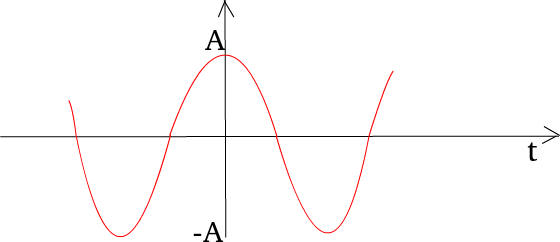
\includegraphics[width=.5\textwidth]{./pictures/2_4.png}
 \caption{Траектория процесса}
 \label{fig:24}
\end{figure}

Тут случайная амплитуда и случайный сдвиг по фазе.

$MX \left( t \right) =
M \left[ A \cos \left( \varphi + \lambda t \right) \right] $.
Случайные величины $A$ и $ \varphi $ --- независимые.
$M \left[ A \cos \left( \varphi + \lambda t \right) \right] =
  MAM \cos \left( \varphi + \lambda t \right) $.
Математическое ожидание косинуса можем найти, потому что у $ \varphi $ известна плотность
$$MAM \cos \left( \varphi + \lambda t \right) =
  MA \cdot \int \limits_0^{2 \pi }
    \cos \left( \varphi + \lambda t \right) \cdot \frac{1}{2 \pi } \cdot d \varphi.$$
Интеграл косинуса по периоду --- ноль.

Ковариационная функция
$K \left( t, s \right) =
  MX \left( t \right) X \left( s \right) - MX \left( t \right) MX \left( s \right) =$
Произведение математических ожиданий мы знаем
$$= MX \left( t \right) X \left( s \right) =
  M \left[
    A^2 \cos \left( \varphi + \lambda t \right) \cos \left( \varphi + \lambda s \right) \right] =$$
Используем независимость
$$= MA^2 \cdot
  M \left[ \cos \left( \varphi + \lambda t \right) \left( \varphi + \lambda s \right) \right] =$$
Применяем формулу для произведения косинусов
$$= MA^2 \cdot M \left\{
    \frac{1}{2} \cdot \cos \left[ 2 \varphi + \lambda \left( t + s \right) \right] +
    \frac{1}{2} \cdot \cos \left[ \lambda \left( t - s \right) \right] \right\} =$$
Математическое ожидание первого слагаемого --- ноль
$$= \frac{1}{2} \cdot MA^2 \cdot \cos \left[ \lambda \left( t - s \right) \right].$$

Двумерная характеристика процесса зависит только от расстояния между двумя точками.
Это стационарный процесс.
Его характеристики не меняются при сдвиге.

\subsubsection*{2.5}

\textit{Задание.}
Пусть $ \tau $ --- случайная величина,
которая имеет равномерное распределение на отрезке $ \left[ 0, 1 \right] $,
и пусть $ \left\{ X \left( t \right), \, t \in \left[ 0, 1 \right] \right\} $ --- процесс ожидания,
связанный с этой случайной величиной, то есть
$$X \left( t \right) =
  \mathbbm{1} \left\{ t \geq \tau \right\}, \,
  t \in \left[ 0, 1 \right].$$
Запишите конечномерные распределения процесса
$ \left\{ X \left( t \right), \, t \in \left[ 0, 1 \right] \right\} $,
найдите его математическое ожидание и ковариационную функцию.

\textit{Решение.}
$ \tau $ --- случайная величина с распределением $U \left( \left[ 0 , 1 \right] \right) $.

Сначала нарисуем траекторию такого процесса (рис. \ref{fig:25}).
Случайное $ \tau $ выпало.

\begin{figure}[h!]
 \centering
 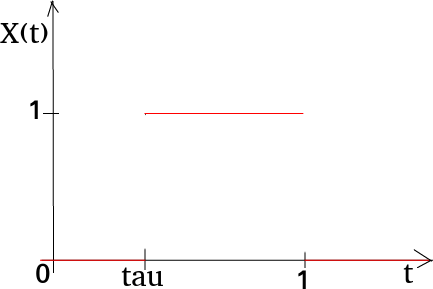
\includegraphics[width=.5\textwidth]{./pictures/2_5.png}
 \caption{Траектория процесса}
 \label{fig:25}
\end{figure}

$$m \left( t \right) =
  MX \left( t \right) =
  M \mathbbm{1} \left\{ t \geq \tau \right\} =
  P \left( t \geq \tau \right) =
  F_{ \tau } \left( t \right) =
  \frac{t - a}{b - a} =
  t.$$

Ковариационная функция
$K \left( t, s \right) =
  M \left[ X \left( t \right) X \left( s \right) \right] -
  MX \left( t \right) MX \left( s \right) $.
Произведение индикаторов --- это индикатор пересечения
$$M \left[ X \left( t \right) X \left( s \right) \right] -
  MX \left( t \right) MX \left( s \right) =
  P \left\{ \tau \leq \min \left( t, s \right) \right\} - ts =
  \min \left( t, s \right) - t \cdot s.$$

Конечномерные распределения ---
распределение вектора $ \left( X \left( t_1 \right), \dotsc, X \left( t_n \right) \right) $.
Каждый $X$ --- это 0 или 1.
$$P \left\{
    \left( X \left( t_1 \right), \dotsc, X \left( t_n \right) \right) = \left( 0, \dotsc, 0 \right)
  \right\} =
  P \left\{ \tau \in \left( t_n , 1 \right] \right\} =
  1 - t_n.$$
Точки $t_n$ изображены на рисунке \ref{fig:251}.

\begin{figure}[h!]
 \centering
 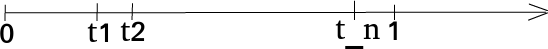
\includegraphics[width=.5\textwidth]{./pictures/2_5_1.png}
 \caption{Временная ось}
 \label{fig:251}
\end{figure}

У вектора получается $ \left( n + 1 \right) $-но значение
$$ \left( X \left( t_1 \right), \dotsc, X \left( t_n \right) \right) =
  \begin{cases}
    \left( 0, \dotsc, 0 \right), \qquad 1 - t_n, \\
    \left( 0, \dotsc, 0, 1 \right), \qquad t_n - t_{n - 1}, \\
    \dotsc, \\
    \left( 0, \dotsc, 0, 1, \dotsc, 1 \right), \qquad t_{k + 1} - t_k, \\
    \dotsc, \\
    \left( 1, \dotsc, 1 \right), \qquad t_1.
  \end{cases}$$

\subsubsection*{2.6}

\textit{Задание.}
Пусть $ \xi_1, \xi_2, \dotsc, \xi_n$ ---
независимые одинаково распределённые случайные величины с функцией распределения $F$, и пусть
$$X \left( t \right) \equiv
  F_n^* \left( t \right) =
  \frac{1}{n} \sum \limits_{i = 1}^n \mathbbm{1} \left\{ \xi_i \leq t \right\}, \,
  t \in \mathbb{R}.$$
Запишите конечномерные распределения процесса
$ \left\{ X \left( t \right), \, t \in \mathbb{R} \right\} $,
найдите его математическое ожидание и ковариационную функцию.

\textit{Решение.}
$$X \left( t \right) =
  \frac{1}{n} \sum \limits_{i = 1}^n \mathbbm{1} \left\{ \xi_i \leq t \right\} $$
--- это эмпирическая функция распределения (рис. \ref{fig:26}).

\begin{figure}[h!]
 \centering
 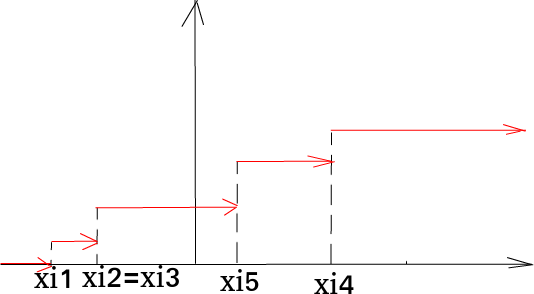
\includegraphics[width=.5\textwidth]{./pictures/2_6.png}
 \caption{Эмпирическая функция распределения}
 \label{fig:26}
\end{figure}

Эмпирическая функция распределения --- это несмещённая оценка функции распределения.

$$cov \left( X \left( t \right), X \left( s \right) \right) =
  cov \left(
    \frac{1}{n} \sum \limits_{i = 1}^n \mathbbm{1} \left\{ \xi_i \leq t \right\}, \,
    \frac{1}{n} \sum \limits_{i = 1}^n \mathbbm{1} \left\{ \xi_i \leq s \right\} \right) =$$
Нужно вынести константы
$$= \frac{1}{n^2}
  \sum \limits_{i,j=1}^n
    cov \left(
      \mathbbm{1} \left\{ \xi_i \leq t, \, \mathbbm{1} \left\{ \xi_j \leq s \right\} \right\}
    \right) =$$
Случайные величины $ \xi_1, \dotsc, \xi_n$ --- независимые.
Ковариация независимых величин --- ноль
$$= \frac{1}{n^2}
  \sum \limits_{i = 1}^n
    \left(
      \mathbbm{1} \left\{ \xi_i \leq t \right\}, \, \mathbbm{1} \left\{ \xi_i \leq s \right\}
    \right).$$

Посчитаем ковариацию двух индикаторов
$$cov \left(
    \mathbbm{1} \left\{ \xi_i \leq t \right\}, \, \mathbbm{1} \left\{ \xi_i \leq s \right\}
  \right) =
  M \mathbbm{1} \left\{ \xi_i \leq t \wedge s \right\} - F \left( t \right) F \left( s \right) =$$
Математическое ожидание индикатора событие --- вероятность этого события,
которая в данном случае по определению равна функции распределения
$$= F \left( t \wedge s \right) - F \left( t \right) F \left( s \right),$$
где $ \wedge $ означает минимум.

Все слагаемые в сумме раны этому выражению
$$K \left( t, s \right) =
  \frac{1}{n} \left[ F \left( t \wedge s \right) - F \left( t \right) F \left( s \right) \right].$$

Теперь нужно написать конечномерные распределения этого процесса.
Фиксируем $t_1, t_2, \dotsc, t_m$ (рис. \ref{fig:261}).

$$X \left( t \right) \in
  \left\{ 0, \frac{1}{n}, \frac{2}{n}, \dotsc, 1 \right\}.$$

По $t, \, X$ увеличивается.
Эта функция монотонна.

\begin{figure}[h!]
 \centering
 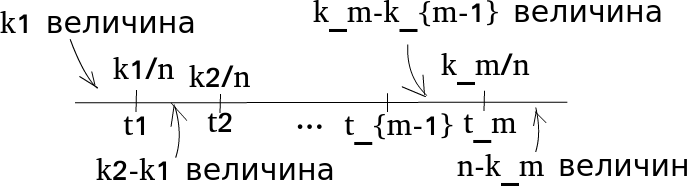
\includegraphics[width=.5\textwidth]{./pictures/2_6_1.png}
 \caption{Фиксируем моменты времени}
 \label{fig:261}
\end{figure}

$0 \leq k_1 \leq k_2 \leq \dotsc \leq k_m \leq n$.

Конечномерные распределения имеют вид
$$P \left\{
    X \left( t_1 \right) = \frac{k_1}{n}, \,
    X \left( t_2 \right) = \frac{k_2}{n}, \dotsc, X \left( t_m \right) = \frac{k_m}{n} \right\} =$$
$P$(для $k_1$ наблюдений $ \xi \leq t_1$, для $k_2 - k_1$ наблюдений $t_1 < \xi \leq t_2, \dotsc,$
для $n - k_m$ наблюдений $ \xi > t_m$)
Имеем мультиномиальное распределение
$$= \frac{n!}{k_1! \left( k_2 - k_1 \right)! \dotsc \left( n - k_m \right)!} \cdot
  F \left( t_1 \right)^{k_1} \cdot
  \left[ F \left( t_2 \right) - F \left( t_1 \right) \right]^{k_2 - k_1} \cdot \dotsc,$$
где первое слагаемое --- количество способов разбить $n$ величин на группы.

\subsubsection*{2.7}

\textit{Задание.}
Найдите характеристическую функцию случайной величины $X \left( \eta \right) $,
где $ \left\{ X \left( t \right), \, t \in \left[ 0, 1 \right] \right\} $ --- процесс из задачи 2.5,
а $ \eta $ --- независимая от $X$ случайная величина,
которая принимает значения 0 и 1 с вероятностями $ \frac{1}{3}$ и $ \frac{2}{3}$ соответственно.

\textit{Решение.}
$X \left( t \right) =
  \mathbbm{1} \left\{ t \geq \tau \right\} $.

Задана случайная величина
$$ \eta =
  \begin{cases}
    0, \qquad \frac{1}{3}, \\
    1, \qquad \frac{2}{3}.
  \end{cases}$$

Интересуемся $ \varphi_{X \left( \eta \right) }$.
Траектория случайного процесса изображён на рисунке \ref{fig:27}.

\begin{figure}[h!]
 \centering
 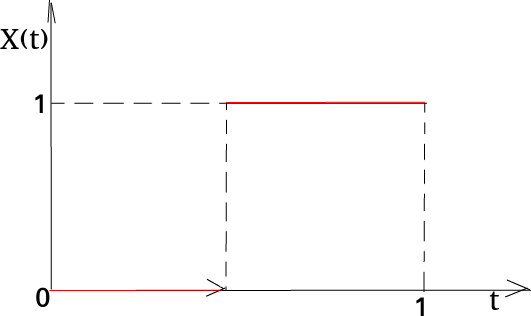
\includegraphics[width=.5\textwidth]{./pictures/2_7.png}
 \caption{Траектория случайного процесса}
 \label{fig:27}
\end{figure}

Случайная величина принимает значения 0 и 1: $X \left( 0 \right) = 0, \, X \left( 1 \right) = 1$,
значит, $X \left( \eta \right) = \eta $.

$$ \varphi_{X \left( \eta \right) } \left( \lambda \right) =
  \varphi_{ \eta } \left( \lambda \right) =
  Me^{i \lambda \eta } =
  \frac{1}{3} \cdot 1 + \frac{2}{3} \cdot e^{i \lambda }.$$

То, что они независимы, тут не важно.

\subsubsection*{2.8}

\textit{Задание.}
Значение случайного телеграфного сигнала
$ \xi = \left\{ \xi \left( t \right) , \,
  t \in \mathbb{R} \right\} $
в произвольный момент времени с одинаковыми вероятностями равно 0 или 1.
Прыжки происходят случайным и независимым образом.
Вероятность $P \left( k, T \right) $ того, что в интервале времени длины $T$ произойдёт $k$ прыжков,
задаётся распределением Пуассона, то есть:
$$P \left( k, T \right) =
  \frac{ \left( \lambda T \right)^k}{k!} \cdot e^{-\lambda T},$$
где $ \lambda $ --- среднее количество прыжков за единицу времени.
Найдите математическое ожидание и ковариационнуб функцию случайного процесса $ \xi $.

\textit{Решение.}
$$P \left\{ \xi \left( t \right) = 1 \right\} =
  P \left\{ \xi \left( t \right) = 0 \right\} =
  \frac{1}{2}.$$
Одномерные распределения даны.
Это распределение Бернулли.

$P \left( k, T \right) $ --- это вероятность того,
что на отрезке времени длины $T$ было $k$ прыжков (распределение Пуассона),
то есть траектория процесса выглядит как на рисунке \ref{fig:28}.

\begin{figure}[h!]
 \centering
 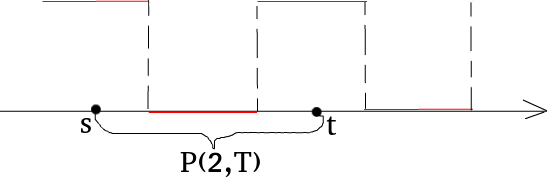
\includegraphics[width=.5\textwidth]{./pictures/2_8.png}
 \caption{Траектория случайного процесса}
 \label{fig:28}
\end{figure}

В каждой точке будет 0 или 1.

Математическое ожидание тут ищется просто
$$M \xi \left( t \right) =
  0 \cdot \frac{1}{2} + 1 \cdot \frac{1}{2} =
  \frac{1}{2}.$$
Теперь нужно ещё найти ковариационную функцию такого процесса
$$K \left( s, t \right) =
  M \left[
    \left( \xi \left( t \right) - M \xi \left( t \right) \right) \cdot
    \left( \xi \left( s \right) - M \xi \left( s \right) \right) \right] =
  M \xi \left( s \right) \xi \left( t \right) - \frac{1}{4}.$$
Нужно математическое ожидание совместного процесса.
$ \xi \left( s \right) $ и $ \xi \left( t \right) $ зависимы.

Попробуем найти математическое ожидание произведения.
$ \xi \left( t \right) \xi \left( s \right) $ принимают значения 0 и 1.
Произведение принимает значения 0 и 1.
Получаем
$$M \xi \left( t \right) \xi \left( s \right) =
  0 \cdot P \left\{ \xi \left( t \right) \xi \left( s \right) = 0 \right\} +
  1 \cdot P \left\{ \xi \left( t \right) \xi \left( s \right) = 1 \right\} =$$
Слагаемое с нулём пропадает
$$= P \left\{ \xi \left( s \right) = 1, \, \xi \left( t \right) = 1 \right\}.$$
Значения в точках совпадаю, если между ними произошло чётное количество скачков
$M \xi \left( t \right) \xi \left( s \right) = P \left\{ \xi \left( s \right) = 1 \right\} P$
(на отрезке $ \left[ s, t \right] $ будет чётное количество прыжков)
$= \frac{1}{2} \cdot P$(на отрезке $ \left[ s, t \right] $ будет чётное число прыжков).
Мы знаем, с какой вероятностью происходит число прыжков.

Подходят любые чётные прыжки, то есть это вероятность объединения.
Число скачков обозначим буковокой $N$.
Тогда $P$(на $ \left[ s, t \right] $ чётное число скачков)
$= P$($N_{ \left[ s, t \right] }$ чётное)$=$
$$ \sum \limits_{k = 0}^{ \infty } P \left( 2k = N_{ \left[ s, t \right] } \right) =
  \sum \limits_{k = 0}^{ \infty } P \left( 2k, t - s \right) =
  \sum \limits_{k = 0}^{ \infty }
    \frac{ \left[ \lambda \left( t - s \right) \right]^{2k}}{ \left( 2k \right)!} \cdot
    e^{-\lambda \left( t - s \right) } =$$
Экспонента выносится за сумму.
Остаётся сумма
$$ \sum \limits_{k = 0}^{ \infty } \frac{x^{2k}}{ \left( 2k \right)!}.$$
Для того, чтобы это было экспонента, нужны ещё и нечётные степени
$$ \sum \limits_{k = 0}^{ \infty } \frac{x^{2k}}{ \left( 2k \right)!} +
  \sum \limits_{k = 0}^{ \infty } \frac{x^{2k + 1}}{ \left( 2k + 1 \right)!} =
  e^x.$$
Если мы вычтем вторую сумму, то получится
$$ \sum \limits_{k = 0}^{ \infty } \frac{x^{2k}}{ \left( 2k \right)!} -
  \sum \limits_{k = 0}^{ \infty } \frac{x^{2k + 1}}{ \left( 2k + 1 \right)!} =
  \sum \limits_{k = 0}^{ \infty } \frac{ \left( -x \right)^{2k}}{ \left( 2k \right)!} +
  \sum \limits_{k = 0}^{ \infty } \frac{ \left( -x \right)^{2k + 1}}{ \left( 2k + 1 \right)!} =
  e^{-x}.$$
Теперь нужно сложить эти два выражения и поделить на 2, то есть
$$ \sum \limits_{k = 0}^{ \infty } \frac{x^{2k}}{ \left( 2k \right)!} =
  \frac{e^x + e^{-x}}{2}, \,
  x = \lambda \left( t - s \right).$$
Получили гиперболический косинус.
$$= \frac{e^{ \lambda \left( t - s \right) } +
  e^{-\lambda \left( t- s \right) }}{2} \cdot e^{-\lambda \left( t - s \right) } =$$
Умножим один сомножитель на другой,
$e^{ \lambda \left( t - s \right) } \cdot e^{-\lambda \left( t -s \right) }$ дают единицу.
Получаем
$$= \frac{1 + e^{-2 \lambda \left( t - s \right) }}{2}.$$
Это вероятность чётного числа скачков.

Выпишем, чему равна ковариационная функция.
Математическое ожидание произведения нужно умножить на $ \frac{1}{2}$ и отнять $ \frac{1}{4}$.
Получится
$$K \left( t, s \right) =
  \frac{1 + e^{-2 \lambda \left( t - s \right) }}{4} - \frac{1}{4} =
  \frac{e^{-2 \lambda \left( t - s \right) }}{4}, \,
  s < t.$$
Окончательный ответ:
$$K \left( t, s \right) =
  \frac{1}{4} \cdot e^{-2 \lambda \left| t - s \right| }.$$

\subsubsection*{2.9}

\textit{Задание.}
Пусть $ \eta_1$ и $ \eta_2$ --- независимые случайные величины,
которые имеют равномерное распределение на отрезке $ \left[ -1, 1 \right] $.
Найдите значения $a$, при которых почти все реализации случайной функции
$t \left( \eta_1 + a \left( \eta_2 + 2a \right) \right) $ монотонно возрастают по $t$.

\textit{Решение.}
$ \xi \left( t \right) = t \left( \eta_1 + a \left( \eta_2 + 2a \right) \right) $ --- процесс.
Известно, что траектория этого процесса монотонно возрастает по $t$.

Реализация такого процесса выглядит как прямая линия (рис. \ref{fig:29}),
при этом $ \eta_1 + a \left( \eta_2 + 2a \right) > 0$.
Это случайная величина, так что
$$P \left\{ \eta_1 + a \left( \eta_2 + 2a \right) > 0 \right\} = 1.$$

\begin{figure}[h!]
 \centering
 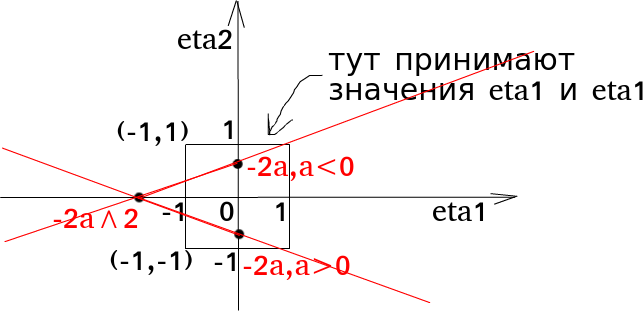
\includegraphics[width=.5\textwidth]{./pictures/2_9.png}
 \caption{Траектория случайного процесса}
 \label{fig:29}
\end{figure}

При $a = 0 \, \eta_1 > 0$ --- правая часть квадратика.
Тогда событие выполняется с вероятностью
$$ \frac{1}{2} \neq 1,$$
то есть $a \neq 0$.

Следующий случай: $a > 0$.
Получается
$$ \eta_2 + 2a >
  -\frac{ \eta_1}{a},$$
откуда
$$ \eta_2 >
  -\frac{ \eta_1}{a} - 2a,$$
то есть на картинке это будет прямая.
Мы возьмём всё, что над этой прямой
$$y =
  -\frac{x}{a} - 2a.$$
Вероятность не будет равна 1.
$a$ должно быть таким, чтобы прямая прошла через точку $ \left( -1, -1 \right) $,
то есть $-1 + a \left( 2a - 1 \right) > 0$.
Теперь можно найти $a$ из неравенства $2a^2 - a - 1 > 0$.
Сейчас скажем, при каких $a$ это выполнено.
$D = 1 + 8 = 9 = 3^2$, значит
$$a_1 = - \frac{1}{2}, \,
  a_2 = 1.$$
Задавали $a > 0$, то есть при $a > 1$ вероятность такого события --- единица.

Теперь нужно задать $a < 0$.
Отличие будет в том, как пройдёт прямая.
$$-\frac{ \eta_1}{a} - 2a >
  \eta_2,$$
то есть нужно нарисовать прямую
$$y =
  -\frac{x}{a} - 2a.$$
Нужно будет выбрать всё, что ниже этой прямой.

Нужно, чтобы прямая прошла над точкой $ \left( -1, 1 \right) $.
Имеем неравенство $-1 + a \left( 1 + 2a \right) > 0$, откуда
$$a^1 + \frac{1}{2} \cdot a - 1 >
  0.$$
Решая соответствующее уравнение находим, что
$$a_1 = \frac{1}{2}, \,
  a_2 = 1.$$
При $a < 0$ получаем ответ: $a < -1$.

Ответ к задаче: $a \in \left( - \infty, -1 \right) \cup \left( 1, + \infty \right) $,
то есть $ \left| a \right| > 1$.

\subsubsection*{2.10}

\textit{Задание.}
Пусть случайная величина $ \tau \in \left( 0, 1 \right) $ имеет непрерывное распределение и пусть
$$ \xi \left( t \right) \equiv 0; \,
  \eta \left( t \right) =
  \begin{cases}
    0, \qquad t \neq \tau, \\
    1, \qquad t = \tau,
  \end{cases} \,
  t \in \left[ 0, 1 \right].$$
Изобразите трактории этих процессов.
Докажите, что эти процессы являются стохастически эквивалентными, то есть
$ \forall t \in \left[ 0, 1 \right] \, : \,
  P \left\{ \xi \left( t \right) \neq \eta \left( t \right) \right\} = 0$.

\textit{Решение.}
$ \tau $ --- это случайная величина с непрерывным распределением --- та,
у которой функция распределения $F_{ \tau }$ --- непрерывна.

Скачок фукнции распределения $ \Delta F_{ \tau } \left( x \right) = P \left( \tau = x \right) = 0$,
где
$$F_{ \tau } \left( x \right) = P \left( \tau \leq x \right),$$
а $F_{ \tau } \left( -x \right) = P \left( \tau < x \right) $.
В нашем случае нет скачков, то есть в фиксированный $x$ случайная величина $ \tau $ не попадёт.
Рассматривается 2 процесса.
Посмотрим, какие траектории у этих процессов.
Процессы заданы на $t \in \left[ 0, 1 \right] $ (рис. \ref{fig:210}).

\begin{figure}[h!]
 \centering
 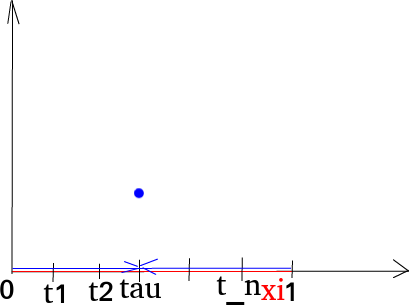
\includegraphics[width=.5\textwidth]{./pictures/2_10.png}
 \caption{Траектория случайных процессов}
 \label{fig:210}
\end{figure}

С точки зрения анализа это разные функции.
У $ \eta $ всегда есть скачок, у $ \xi $ никогда скачков нет.
Помним, что $ \xi \left( t \right) \equiv 0$.
Тем не менее, вероятность
$P \left\{ \xi \left( t \right) \neq \eta \left( t \right) \right\} =
  P \left\{ \eta \left( t \right) \neq 0 \right\} =
  P \left( \tau = t \right) =
  0$,
а это значит, что в фиксированной точке процессы с вероятностью 1 совпадают.
Если зафиксируем несколько точек $t_1, t_2, \dotsc, t_n$, то вероятность
$$P \left\{
    \left( \xi \left( t_1 \right), \dotsc, \xi \left( t_n \right) \right) =
    \left( \eta \left( t_1 \right), \dotsc, \eta \left( t_n \right) \right) \right\} =
  1.$$
У этих процессов одинаковые конечномерные распределения.

Конечномерные распределения не определяют траектории процесса.

\addcontentsline{toc}{section}{Домашнее задание}
\section*{Домашнее задание}

\subsubsection*{2.12}

\textit{Задание.}
Пусть
$$ \xi \left( t \right) =
  Xt + a, \,
  t \in \mathbb{R},$$
где $X$ --- равномерно распределённая на отрезке $ \left( a, b \right) $ случайная величина.
Запишите конечномерные распределения случайного процесса
$ \left\{ \xi \left( t \right), \, t \in \mathbb{R} \right\} $.
Найдите его математическое ожидание, дисперсию и ковариационную функцию.

\textit{Решение.}
$ \xi \left( t \right) = Xt + a, \, t \in \mathbb{R}$, где $X \sim U \left( a, b \right) $.

Нужно найти $m \left( t \right), \, D \xi \left( t \right), \, K \left( t, s \right) $,
конечномерные распределения.

Найдём математическое ожидание в момент $t$
$$m \left( t \right) =
  M \xi \left( t \right) =
  M \left( Xt + a \right) =
  M \left( Xt \right) + Ma =
  tMX + a =
  t \cdot \frac{a + b}{2} + a.$$

Траектории такого процесса изоражены на рисунке \ref{fig:212}: чем больше $X$,
тем больше угол наклона прямой к оси $0t$.

\begin{figure}[h!]
 \centering
 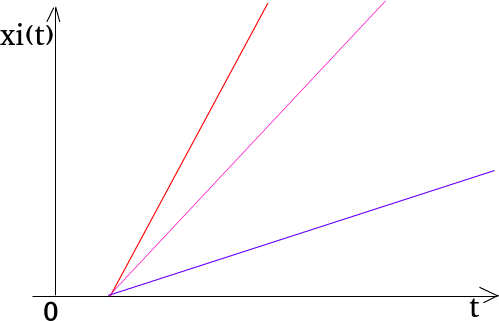
\includegraphics[width=.5\textwidth]{./pictures/2_12.png}
 \caption{Траектории случайного процесса}
 \label{fig:212}
\end{figure}

$$D \xi \left( t \right) =
  D \left( Xt + a \right) =
  D \left( Xt \right) + Da =
  t^2 DX =
  t^2 \cdot \frac{ \left( b - a \right)^2}{12}.$$

Ковариационная функция считается по определению
$$K \left( t, s \right) =
  M \left[ \xi \left( t \right) \xi \left( s \right) \right] -
  M \xi \left( t \right) M \xi \left( s \right) =$$
Подставляем выражение для случайного процесса, раскрываем скобки и вычисляем математическое ожидание
\begin{equation*}
  \begin{split}
    = M \left[ \left( Xt + a \right) \left( Xs + a \right) \right] -
    M \left( Xt + a \right) M \left( Xs + a \right) = \\
    = M \left[ X^2 ts + Xa \left(t + s \right) + a^2 \right] -
    \left( t \cdot \frac{a + b}{2} + a \right) \left( s \cdot \frac{a + b}{2} + a \right) = \\
    = ts \cdot \frac{a^2 + ab + b^2}{3} + a \left( t + s \right) \cdot \frac{a + b}{2} + a^2 -
    ts \cdot \frac{ \left( a + b \right)^2}{4} - ta \cdot \frac{a + b}{2} - a^2 - \\
    - as \cdot \frac{a + b}{2} = \\
    = ts \left( \frac{a^2 + ab + b^2}{3} - \frac{a^2 + 2ab + b^2}{4} \right) +
    \left(t + s \right) a \cdot \frac{a + b}{2} - \frac{a + b}{2} \cdot a \left( t + s \right) = \\
    = ts \cdot \frac{4a^2 + 4ab + 4b^2 - 3a^2 - 6ab - 3b^2}{12} =
    ts \cdot \frac{a^2 - 2ab + b^2}{12} =
    ts \cdot \frac{ \left( a - b \right)^2}{12}.
  \end{split}
\end{equation*}

Считаем функцию распределения случайного вектора
$ \left( \xi \left( t_1 \right), \dotsc, \xi \left( t_n \right) \right) $ --- рис. \ref{fig:2121}.

\begin{figure}[h!]
 \centering
 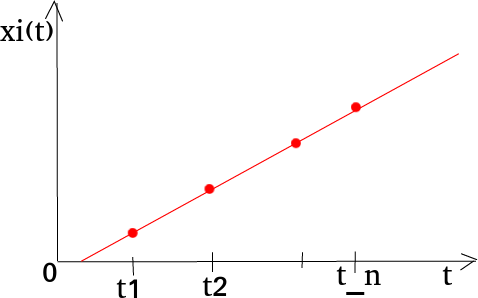
\includegraphics[width=.5\textwidth]{./pictures/2_12_1.png}
 \caption{Выбираем точки, в которых ищем распределение случайного процесса}
 \label{fig:2121}
\end{figure}

$F_{ \left( \xi \left( t_1 \right), \dotsc, \xi \left( t_n \right) \right) }
  \left( \vec{x} \right) =
  P \left\{ \xi \left( t_1 \right) \leq x_1, \dotsc, \xi \left( t_n \right) \leq x_n \right\} $.
Вместо $ \xi $ напишем формулу
$P \left\{ \xi \left( t_1 \right) \leq x_1, \dotsc, \xi \left( t_n \right) \leq x_n \right\} =
  P \left( Xt_1 + a \leq x_1, \dotsc, Xt_n + a \leq x_n \right) $.
Величины зависимы, потому что все они выражаются через $X$.
Все неравенства решаем относительно $X$
$$P \left( Xt_1 + a \leq x_1, \dotsc, Xt_n + a \leq x_n \right) =
  P \left( Xt_1 \leq x_1 - a, \dotsc, Xt_n \leq x_n - a \right) =$$
Делим на константы левые части неравенств
$$= P \left( X \leq \frac{x_1 - a}{t_1}, \dotsc, X \leq \frac{x_n - a}{t_n} \right) =$$
Перепишем через минимум
$$= P \left\{
    X \leq \min \left( \frac{x_1 - a}{t_1}, \dotsc, \frac{x_n - a}{t_n} \right)
  \right\} =$$
Обозначим минимум буквой $m$ для удобства
$$= P \left( X \leq m \right) =
  \int \limits_a^m \frac{1}{b - a} \cdot \mathbbm{1} \left\{ X \in \left( a, b \right) \right\} dX =
  \frac{1}{b - a} \int \limits_a^m dX =
  \frac{1}{b - a} \cdot \left. X \right|_a^m =$$
Подставляем пределы интегрирования
$$= \frac{1}{b - a} \cdot \left( m - a \right) =
  \frac{1}{b - a} \cdot
  \left[ \min \left( \frac{x_1 - a}{t_1}, \dotsc, \frac{x_n - a}{t_n} \right) - a \right] $$
при $m \in \left( a, b \right) $, иначе --- ноль.

\subsubsection*{2.13}

\textit{Задание.}
Пусть
$$ \xi \left( t \right) =
  U \cos \theta t + V \sin \theta t, \,
  t \in T,$$
где $U, V$ --- независимые случайные величины с заданными характеристиками:
$MU = MV = 0, \, DU = DV = \sigma^2, \, \theta $ --- неслучайная величина.
Найдите математическое ожидание, дисперсию и ковариационную функцию случайного процесса
$ \left\{ \xi \left( t \right), \, t \in T \right\} $.

\textit{Решение.}
Нужно найти $m \left( t \right), \, D \xi \left( t \right), \, K \left( t, s \right) $.

Найдём математическое ожидание в момент $t$.
По свойствам
$$m \left( t \right) =
  M \xi \left( t \right) =
  M \left( U \cos \theta t + V \sin \theta t \right) =
  \cos \theta t \cdot MU + \sin \theta t \cdot MV =
  0.$$

Можно сделать преобразование
$U \cos \theta t + V \sin \theta t = C \sin \left( \theta t + \omega \right) $,
где $C = \sqrt{U^2 + V^2}$.
Траектории такого процесса изображены на рисунке \ref{fig:213}:
график синуса сжимается к оси ординат, когда модули случайных величин $U$ и $V$ растут.

\begin{figure}[h!]
 \centering
 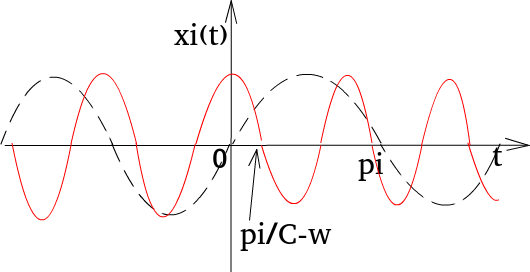
\includegraphics[width=.5\textwidth]{./pictures/2_13.png}
 \caption{Траектория процесса}
 \label{fig:213}
\end{figure}

Найдём дисперсию в момент $t$.
По свойствам
$$D \xi \left( t \right) =
  D \left( U \cos \theta t + V \sin \theta t \right) =
  \cos^2 \theta  t \cdot DU + \sin^2 \theta t \cdot DV =$$
Подставим известные значения дисперсии
$$= \cos^2 \theta t \cdot \sigma^2 + \sin^2 \theta t \cdot \sigma^2 =
  \sigma^2 \left( \cos^2 \theta t + \sin^2 \theta t \right) =
  \sigma^2.$$

Ковариационная функция считается по определению
$$K \left( t, s \right) =
  M \xi \left( t \right) \xi \left( s \right) - M \xi \left( t \right) M \xi \left( s \right) =$$
Подставим выражения для случайного процесса в первое слагаемое, а второе равно нулю
$$= M \left[ \left( U \cos \theta t + V \sin \theta t \right) \cdot
    \left( U \cos \theta s + V \sin \theta s \right) \right] =$$
Раскроем скобки
\begin{equation*}
  \begin{split}
    = M(
      U^2 \cos \theta t \cdot \cos \theta s + UV \cos \theta t \cdot \sin \theta s +
      VU \sin \theta t \cdot \cos \theta
       s + \\
      + V^2 \sin \theta t \cdot \sin \theta s) = \\
    = DU \cdot \cos \theta t \cdot \cos \theta s +
    MU \cdot MV \cdot \cos \theta t \cdot \sin \theta s +
    MV \cdot MU \cdot \sin \theta t \cdot \cos \theta s + \\
    + DV \cdot \sin \theta t \cdot \sin \theta s =
    \sigma^2 \cos \theta t \cdot \cos \theta s + \sigma^2 \sin \theta t \cdot \sin \theta s = \\
    = \sigma^2 \cdot
      \left( \cos \theta t \cdot \cos \theta s + \sin \theta t \cdot \sin \theta s \right) =
    \sigma^2 \cos \left( \theta t - \theta s \right) =
    \sigma^2 \cos \left[ \theta \left( t - s \right) \right].
  \end{split}
\end{equation*}

\subsubsection*{2.14}

\textit{Задание.}
Определите математическое ожидание, дисперсию и ковариационную функцию процесса
$$ \xi \left( t \right) =
  2u \sin \nu t + 3vt^2 + 5, \,
  t \in T,$$
где $ \nu $ --- известный неслучайный параметр, а $u, v$ ---
случайные величины с известными характеристиками:
$$Mu = 1, \,
  Mv = 2, \,
  Du = 0.1, \,
  Dv = 0.9, \,
  cov \left( u, v \right) = -0.3.$$

\textit{Решение.}
Нужно найти $m \left( t \right), \, D \xi \left( t \right), \, K \left( t, s \right) $.

Найдём математическое ожидание в момент $t$.
По свойствам
$$m \left( t \right) =
  M \left( 2u \sin \nu t + 3vt^2 + 5 \right) =
  2 \sin \nu t \cdot Mu + 3t^2 Mv + 5 =
  2 \sin \nu t + 6t^2 + 5.$$

Траектория такого процесса изображена на рисунке \ref{fig:214} при $ \nu = 1, \, u = 1, \, v = 2$.

\begin{figure}[h!]
 \centering
 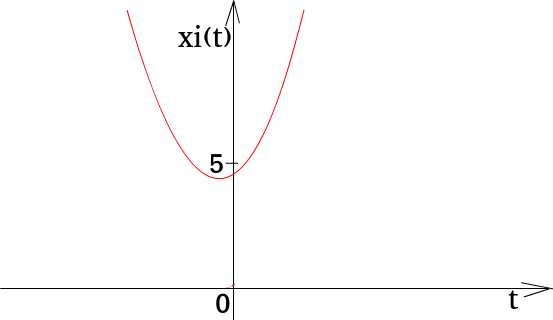
\includegraphics[width=.5\textwidth]{./pictures/2_14.png}
 \caption{Траектория процесса}
 \label{fig:214}
\end{figure}

Ковариационная функция считается по определению
$$K \left( t, s \right) =
  M \xi \left( t \right) \xi \left( s \right) -
    M \xi \left( t \right) \cdot M \xi \left( s \right) =$$
Подставим выражения для случайного процесса и его математические ожидания
\begin{equation*}
  \begin{split}
    = M \left[
      \left( 2u \sin \nu t + 3vt^2 + 5 \right) \left( 2u \sin \nu s + 3vs^2 + 5 \right) \right] - \\
    - \left( 2 \sin \nu t + 6t^2 + 5 \right) \left( 2 \sin \nu s + 6s^2 + 5 \right) = \\
    = M(4u^2 \sin \nu t \cdot \sin \nu s + 6uv \sin \nu t \cdot s^2 + 10u \sin \nu t +
      6vt^2 u \sin \nu s + 9v^2 t^2 s^2 + \\
      + 15vt^2 + 10u \sin \nu s + 15vs^2 + 25) -
    4 \sin \nu t \cdot \sin \nu s - 12 \sin \nu t \cdot s^2 - 10 \sin \nu t - \\
    - 12t^2 \sin \nu s - 36t^2 s^2 - 30t^2 - 10 \sin \nu s - 30s^2 - 25 = \\
    = 4 \sin \nu t \cdot Mu^2 + 6t^2 \sin \nu s \cdot M \left( uv \right) + 10 \sin \nu t \cdot Mu +
    6t^2 \sin \nu s \cdot M \left( uv \right) + \\
    + 9t^2 s^2 Mv^2 + 15t^2 Mv + 10 \sin \nu s \cdot Mu + 15s^2 \cdot Mv + 25 -
    4 \sin \nu t \cdot \sin \nu s - \\
    - 12 \sin \nu t \cdot s^2 - 10 \sin \nu t - 12t^2 \sin \nu s - 36t^2 s^2 - 30t^2 -
    10 \sin \nu s - 30s^2 - 25 =
  \end{split}
\end{equation*}
Вычислим вторые моменты
$$Mu^2 = Du + \left( Mu \right)^2 = 0.1 + 1 = 1.1, \,
  Mv^2 = Dv + \left( Mv \right)^2 = 0.9 + 4 = 4.9.$$
По определению ковариации $cov \left( u, v \right) = M \left( uv \right) - Mu \cdot Mv$,
откуда
$$M \left( uv \right) =
  cov \left( u, v \right) + Mu \cdot Mv =
  -0.3 + 1 \cdot 2 =
  2 - 0.3 =
  1.7.$$
Подставим полученные значения в функцию ковариации
\begin{equation*}
  \begin{split}
    = 4 \sin \nu t \cdot \sin \nu s \cdot 1.1 + 6 \sin \nu t \cdot s^2 \cdot 1.7 + 10 \sin \nu t +
    6t^2 \sin \nu s \cdot 1.7 + \\
    + 9t^2 s^2 \cdot 4.9 + 15t^2 \cdot 2 + 10 \sin \nu s + 15s^2 \cdot 2 -
    4 \sin \nu t \cdot \sin \nu s - 12 \sin \nu t \cdot s^2 - \\
    - 10 \sin \nu t - 12t^2 \cdot \sin \nu s - 36t^2 s^2 - 30t^2 - 10 \sin \nu s - 30s^2 = \\
    = 0.4 \sin \nu t \cdot \sin \nu s - 1.8 \sin \nu t \cdot s^2 - 1.8t^2 \sin \nu s + 8.1t^2 s^2.
  \end{split}
\end{equation*}

Найдём дисперсию в момент $t$.
Из формулы для ковариации
$$D \xi \left( t \right) =
  K \left( t, t \right) =
  0.4 \sin^2 \nu t - 3.6 \sin \nu t \cdot t^2 + 8.1t^4.$$

\subsubsection*{2.15}

\textit{Задание.}
Найдите ковариационную функцию процесса
$$Y \left( t \right) =
  \psi_1 \left( t \right) X_1 + \dotsc + \psi_n \left( t \right) X_n,$$
где $ \psi_1, \dotsc, \psi_n$ --- произвольные числовые функции от $t$, а $X_1, \dotsc, X_n$ ---
некоррелируемые случайные величины с дисперсиями $D_1, \dotsc, D_n$.

\textit{Решение.}
Нужно найти
$$K \left( t, s \right) =
  cov \left( \psi_1 \left( t \right) X_1 + \dotsc + \psi_n \left( t \right) X_n, \,
    \psi_1 \left( s \right) X_1 + \dotsc + \psi_n \left( s \right) X_n \right) =$$
Распишем по определению
\begin{equation*}
  \begin{split}
    = M \left[
      \left( \psi_1 \left( t \right) X_1 + \dotsc + \psi_n \left( t \right) X_n \right)
      \left( \psi_1 \left( s \right) X_1 + \dotsc + \psi_n \left( s \right) X_n \right) \right] - \\
    - M \left( \psi_1 \left( t \right) X_1 + \dotsc + \psi_n \left( t \right) X_n \right) \cdot
    M \left( \psi_1 \left( s \right) X_1 + \dotsc + \psi_n \left( s \right) X_n \right) = \\
    = \sum \limits_{i, j = 1}^n
      \psi_i \left( t \right) \psi_j \left( s \right) M \left( X_i X_j \right) -
    \sum \limits_{i, j = 1}^n \psi_i \left( t \right) \psi_j \left( s \right) MX_i \cdot MX_j = \\
    = \psi_1 \left( t \right) \psi_1 \left( s \right) DX_1 + \dotsc +
    \psi_n \left( t \right) \psi_n \left( s \right) DX_n= \\
    = \psi_1 \left( t \right) \psi_1 \left( s \right) D_1 + \dotsc +
    \psi_n \left( t \right) \psi_n \left( s \right) D_n.
  \end{split}
\end{equation*}

\subsubsection*{2.16}

\textit{Задание.}
Пусть $ \eta $ и $ \zeta $ --- независимые нормально распределённые
случайные величины с нулевым математическим ожиданием и дисперсиями $1 / 2$.
Найдите конечномерные распределения случайного процесса
$$ \xi \left( t \right) =
  \frac{ \eta + \zeta }{t}, \,
  t > 0.$$

\textit{Решение.}
Для произвольных натуральных $n \geq 1$,
произвольных моментов времени $t_1, \dotsc, t_n \in T$ и произвольных действительных чисел
$x_1, \dotsc, x_n$ находим
$$F_{t_1, t_2, \dotsc, t_n} \left( x_1, x_2, \dotsc, x_n \right) =
  P \left\{
    \xi \left( t_1 \right) \leq x_1, \xi \left( t_2 \right) \leq x_2, \dotsc,
    \xi \left( t_n \right) \leq x_n \right\} =$$
Подставляем выражения для случайного процесса
$$= P \left(
    \frac{ \eta + \zeta }{t_1} \leq x_1, \frac{ \eta + \zeta }{t_2} \leq x_2, \dotsc,
    \frac{ \eta + \zeta }{t_n} \leq x_n \right) =$$
Переносим моменты времени вправо
$$= P \left(
    \eta + \zeta \leq x_1 t_1, \eta + \zeta \leq x_2 t_2, \dotsc, \eta + \zeta \leq x_n t_n
  \right) =$$
Независимые случайные величины $ \eta $ и $ \zeta $ имеют нормальное распределение с параметрами
$a = 0$ и
$$ \sigma^2 =
  \frac{1}{2}.$$
Их сумма имеет стандартное нормальное распределение.
Пусть
$$ \eta + \zeta =
  X \sim
  N \left( 0, 1 \right).$$
Тогда
$$= P \left( X \leq x_1 t_1, X \leq x_2 t_2, \dotsc, X \leq x_n t_n \right) =
  P \left( X \leq \min \limits_{i = \overline{1, n}} x_i t_i \right) =$$
Запишем через плотность
$$= \int \limits_{- \infty }^z \frac{1}{ \sqrt{2 \pi }} \cdot e^{- \frac{y^2}{2}} dy,$$
где обозначено
$$z =
  \min \limits_{i = \overline{1, n}} x_i t_i.$$

\subsubsection*{2.17}

\textit{Задание.}
Найдите характеристическую функцию случайной величины $ \xi \left( \tau \right) $,
где $ \left\{ \xi \left( t \right),\ , t \geq 0 \right\} $ --- процесс из предыдущей задачи,
а $ \tau $ --- независимая от $ \xi $ случайная величина,
которая принимает значения $+1$ и $-1$ с вероятностями $1 / 2$.

\textit{Решение.}
$$ \xi \left( t \right) =
  \frac{ \eta + \zeta }{t}.$$

Задана случайная величина
$$ \tau =
  \begin{cases}
    1, \qquad \frac{1}{2}, \\
    -1, \qquad \frac{1}{2}.
  \end{cases}$$

Интересует
$$ \varphi_{ \xi \left( \tau \right) } \left( \lambda \right) =
  Me^{i \xi \left( \tau \right) \lambda } =
  Me^{i \cdot \frac{ \eta + \zeta }{ \tau } \cdot \lambda } =$$
Как и в предыдущей задаче $ \eta + \zeta = X \sim N \left( 0, 1 \right) $.
Получаем
$$= Me^{i \cdot \frac{X}{ \tau } \cdot \lambda } =
  Me^{-\frac{ \lambda ^2}{2 \tau^2}} =
  e^{- \frac{ \lambda^2}{2}}.$$

\subsubsection*{2.18}

\textit{Задание.}
Пусть $ \xi $ и $ \eta $ --- случайные величины,
причём $ \eta $ имеет симметричное относительно нуля распределение и
$P \left( \eta = 0 \right) =
  0$.
Найдите вероятность того, что реализации случайного процесса
$ \zeta \left( t \right) = \xi + t \left( \eta + t \right), \, t \geq 0$ возрастают.

\textit{Решение.}
Известно, что траектории процесса возрастают по $t$ при $t \geq 0$.

Реализация такого процесса выглядит как парабола (рис. \ref{fig:218}) с вершиной в точке с координатами
$$t_0 = -\frac{ \eta }{2 \xi }, \,
  \zeta_0 = t_0^2 + \eta t_0 + \xi = \frac{ \eta^2}{4 \xi^2} - \frac{ \eta^2}{2 \xi }  + \xi.$$

\begin{figure}[h!]
 \centering
 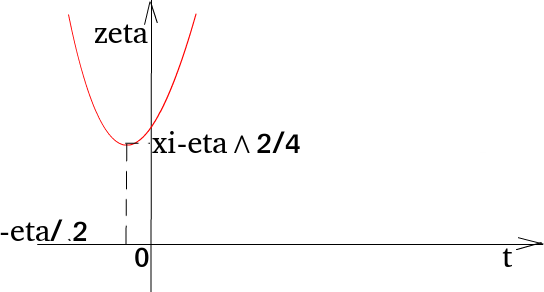
\includegraphics[width=.5\textwidth]{./pictures/2_18.png}
 \caption{Траектория процесса}
 \label{fig:218}
\end{figure}

Это случайная величина, так что
$$P \left\{ \zeta \left( t \right) \geq 0, \, t \geq 0 \right\} =
  P \left\{ \xi + t \left( \eta + t \right) \geq 0, \, t \geq 0 \right\} =$$
$=P$(вершина параболы $ \zeta = t^2 + \eta t + \xi $ лежит слева от нуля)$=$
$$= P \left( -\frac{ \eta }{2 \xi } \leq 0 \right) =
  P \left( \eta \geq 0 \right) =$$
Случайная величина $ \eta $ имеет симметричное распределение
$$= \frac{1}{2}.$$

\subsubsection*{2.19}

\textit{Задание.}
Случайный эксперимент состоит в двухразовом подбрасывании монеты.
Обозначим через $ \omega = \left( \omega_1, \omega_2 \right) $
результат эксперимента и обозначим процессы $ \left\{ X \left( t \right), \, 0 \leq t < 2 \right\} $
и $ \left\{ Y \left( t \right), \, 0 \leq t < 2 \right\} $ следующим образом:
\begin{equation*}
  \begin{split}
    X \left( t \right) =
    \mathbbm{1}_{ \left[ 0, 1 \right) } \left( t \right) \cdot
    \mathbbm{1} \left\{ \omega_1 = P \right\} +
    \mathbbm{1}_{ \left[ 1, 2 \right) } \left( t \right) \cdot
    \mathbbm{1} \left\{ \omega_2 = P \right\}, \,
    0 \leq t < 2, \, \\
    Y \left( t \right) = 1 - X \left( t \right), \, 0 \leq t < 2.
  \end{split}
\end{equation*}
Докажите, что процессы $X \left( t \right) $ и $Y \left( t \right) $
имеют одинаковые конечномерные распределения, но не являются стохастически эквивалентными.

\textit{Решение.}
Рассматривается 2 процесса.
Процессы заданы на $t \in \left[ 0, 2 \right) $.

Это разные функции.
Вероятность
$$P \left\{ X \left( t \right) \neq Y \left( t \right) \right\} =
  P \left\{ X \left( t \right) \neq 1 - X \left( t \right) \right\} =
  1,$$
а это значит, что процессы с вероятностью 1 не совпадают.
Зафиксируем несколько точек $t_1, t_2, \dotsc, t_n$.
Обозначим через $t_{i1}, t_{i2}, \dotsc, t_{ik}$ моменты $t$, которые лежат между 0 и 1,
и $t_{j1}, t_{j2}, \dotsc, t_{j \left( n - k \right) }$ --- все остальные.
Найдём вероятность
\begin{equation*}
  \begin{split}
    P \left\{ X \left( t_1 \right) = x_1, \dotsc, X \left( t_n \right) = x_n \right\} = \\
    = P \left\{X \left( t_{i1} \right) = x_{i1}, \dotsc, X \left( t_{ik} \right) = x_{ik},
        X \left( t_{j1} \right) = x_{j1}, \dotsc, \right. \\
        \left. X \left( t_{j \left( n - k \right) } \right) = x_{j \left( n - k \right) }
      \right\} = \\
    = P \left(
      \mathbbm{1} \left\{ \omega_1 = P \right\} = x_{i1}, \dotsc,
      \mathbbm{1} \left\{ \omega_1 = P \right\} = x_{ik}, \right. \\
      \left. \mathbbm{1} \left\{ \omega_2 = P \right\} = x_{j1}, \dotsc,
      \mathbbm{1} \left\{ \omega_2 = P \right\} = x_{j \left( n - k \right) } \right).
  \end{split}
\end{equation*}
Рассматриваем только случай, когда $x_{i1}, \dotsc, x_{ik}$ одинаковые, и
$$x_{j1}, \dotsc, x_{j \left( n - k \right)}$$
одинаковые.
$$P \left\{ X \left( t_1 \right) = x_1, \dotsc, X \left( t_n \right) = x_n \right\} =
  \frac{1}{2} \cdot \frac{1}{2} =
  \frac{1}{4}.$$

Аналогично
$$P \left\{ Y \left( t_1 \right) = x_1, \dotsc, Y \left( t_n \right) = x_n \right\} =
  \frac{1}{4}.$$

У этих процессов одинаковые конечномерные распределения.
